\documentclass[preprint,12pt]{elsarticle}
\journal{Journal of Computer Languages}

\usepackage{amsmath, amssymb, amsthm,tikz, subfig}
\usetikzlibrary{positioning,shapes,quotes,calc}

\newtheorem{theorem}{Theorem}[section]
\newtheorem{corollary}{Corollary}[theorem]
\newtheorem{lemma}{Lemma}[section]
\theoremstyle{definition}
\newtheorem{definition}{Definition}[section]
\newtheorem{example}{Example}[section]
\theoremstyle{remark}
\newtheorem{remark}{Remark}[section]

\usepackage{algorithm, algpseudocode}
\algrenewcommand\algorithmicrequire{\textbf{Input:}}
\algrenewcommand\algorithmicensure{\textbf{Output:}}

\usepackage{scalerel}
\DeclareMathOperator*{\bigplus}{\scalerel*{+}{\sum}}

\usepackage[strings]{underscore} % fixes doi underscores
\usepackage{hyperref} % brings up so many errors
\usepackage[capitalise, noabbrev]{cleveref}

\newcommand{\AP}{\mathcal{AP}}
\newcommand{\always}{\Box}
\newcommand{\eventually}{\Diamond}
\newcommand{\nextt}{\mathcal{X}}
\newcommand{\limplies}{\rightarrow}
\newcommand{\ltl}{\textit{LTL}}

\newcommand{\Buchi}{B\"{u}chi }
\newcommand{\stronguntil}{\hspace{0.1cm} \mathcal{U}  \hspace{0.1cm}}
\newcommand{\strongrelease}{\hspace{0.1cm} \mathcal{M} \hspace{0.1cm}}
\newcommand{\weakuntil}{\hspace{0.1cm} \mathcal{W} \hspace{0.1cm}}
\newcommand{\weakrelease}{\hspace{0.1cm} \mathcal{R} \hspace{0.1cm}}
\newcommand{\liff}{\leftrightarrow}

\newcommand{\tool}{\hspace{0.1cm}\texttt{ltl2timeline}\hspace{0.1cm}}

\newcommand{\tllen}{\text{tllen}}

\begin{document}

\begin{frontmatter}
    \title{What's in a Name? Linear Temporal Logic Literally Represents Time Lines}

	\author[inst1]{Runming Li\corref{cor1}}
    \ead{runmingl@andrew.cmu.edu}

	\author[inst1]{Keerthana Gurushankar\corref{cor1}}
    \ead{kgurusha@andrew.cmu.edu}

    \author[inst1]{Marijn~J.H.~Heule\corref{cor2}}
    \ead{marijn@cmu.edu}

    \author[inst2]{Kristin~Y.~Rozier}
    \ead{kyrozier@iastate.edu}

    \affiliation[inst1]{organization={Carnegie Mellon University},%Department and Organization
                addressline={5000 Forbes Ave},
                city={Pittsburgh},
                postcode={15213},
                state={PA},
                country={USA}}

    \affiliation[inst2]{organization={Iowa State University},%Department and Organization
                %addressline={Address Two},
                city={Ames},
                postcode={50010},
                state={IA},
                country={USA}}

	\cortext[cor1]{These authors contributed equally to this work}
    \cortext[cor2]{Corresponding author}

    \begin{abstract}
        Linear Temporal Logic (\ltl) is widely used to specify requirements in safety-critical systems.
        However, like many formal verification techniques, it is known to be unintuitive and error-prone for human practitioners to specify and validate.
        In this paper, we provide a new timeline tool for visualizing \ltl-based specifications, which is effective at intuitively representing a wide range of formulas.
        Our tool generates timeline visualizations by translating \ltl\ formulae to intermediate representations as \Buchi automata and then $\omega$-regular expressions, and finally simplifying and visualizing the expressions.
        We provide an algorithm for this visualization, a theoretical soundness analysis, and an implementation.
    \end{abstract}

    \begin{highlights}
        \item We transform Linear Temporal Logic (LTL) formulas to timeline visualizations for the set of satisfying traces.
        \item We translate LTL formulas to \Buchi automata, then to $\omega$-regular expressions, then simplify them and use graph visualization tools to draw timelines.
        \item Our algorithm is sound and complete.
        \item Our tool, \tool, effectively constructs small timeline visualizations for a range of LTL formulas.
    \end{highlights}

    \begin{keyword}
        Modal and Temporal Logics
        \sep Logic and Verification
        \sep Regular languages
    \end{keyword}
\end{frontmatter}
\section{Introduction}

Requirement specification is a central step in the development of safety-critical systems. As a first step, requirements are typically written in natural language. For example, here is a real-world requirement specification from an air traffic control system ~\cite{ZR14}
\begin{center}
    ``If a TSAFE command is sent to an aircraft, controller/AutoResolver should then hand off the control of this aircraft''
\end{center}
Such natural language requirements are often ambiguous and not amenable to formal analysis, so requirements must often be specified using rigorous formalized semantics for the purpose of verification and validation. The above requirement, when translated to Linear Temporal Logic (detailed in \cref{sec:ltl}), may be expressed as follows:
\begin{align*}
    \always (\texttt{tsafe.TSAFE\_command1} \land \texttt{controller.CTR\_control\_1} \\
    \limplies \nextt (\neg \texttt{controller.CTR\_control\_1}))
\end{align*}
Several tools have been developed to reason about formal specifications written with such \ltl\ formulas, like R2U2 and FRET \cite{GPMS20}. However, these formalized semantics are unintuitive and error-prone for human practitioners, and the tools are much less useful when system designers can't validate input specifications.
Thus, a significant hurdle remains: how can we convincingly demonstrate to the humans in the loop, from system designers to certifiers, that the analyzed formulas truly represent the desired system requirements? % quote MLTL paper?

We take a simple idiomatic approach to address this problem. As Linear Temporal Logic formulas are temporal information, we devise a tool, \tool, which can draw timelines to depict the satisfying traces of the \ltl\ formula, and thereby represent the specified behavior in a more natural human-intelligible form.

Our tool, \tool, uses a remarkably simple algorithm: transforming an input \ltl\ formula through a sequence of automaton and regular expression-based intermediate representations, and is surprisingly effective at providing small representations for a range of \ltl\ formulas. It would visualize the above air traffic control requirement behavior with the timeline shown in \cref{example:air}.

We make the following contributions in our paper:
\begin{itemize}
    \item We provide the tool, \tool, which takes \ltl\ formulas and synthesizes timeline visualizations for them.
    \item We prove correctness in \cref{sec:analysis}. We show that for every \ltl\ formula, the timeline outputted indeed represents the set of satisfying traces.
    \item We showcase the results of our tool on a range of example formulas in \cref{sec:tool-showcase} and \cref{sec:playing}, including discussing the air traffic example above.
\end{itemize}

\section{Setting the stage}

We must begin by setting up the prerequisite definitions involved in our work.
First, we provide the definition and semantics for \ltl. In the following subsections, we define (state-based) \Buchi automata and $\omega$-regular expressions, which are generalizations of the well-known deterministic finite automata (DFAs) and regular expressions, for the case of infinite words. Lastly, we describe the graphic visualizations we will use to depict timelines.

\subsection{Linear temporal logic (LTL)} \label{sec:ltl}

\begin{definition}[Linear Temporal Logic (LTL)]
    % cite Kristin's survey paper
    The syntax of an LTL formula over a set of atomic propositions $\AP$, where $p\in\AP$ is a propositional variable, is given by the following grammar:
    \begin{align*}
        \Phi ::= p \mid \neg \Phi \mid \Phi \land \Phi \mid \Phi \lor \Phi \mid \Phi \limplies \Phi \mid \always \Phi \mid \eventually \Phi \mid \nextt \Phi \mid \Phi \stronguntil \Phi \mid \Phi \weakrelease \Phi
    \end{align*}\label{ltl-defn}
\end{definition}

\begin{remark}
    Intuitively, $\always \Phi$ says that formula $\Phi$ is true at every time step; $\eventually \Phi$ says that formula $\Phi$ is true either now or at sometime in the future time step; and $\nextt \Phi$ says formula $\Phi$ is true at the next time step immediately after the current one; $\Phi \stronguntil \Psi$ says that formula $\Phi$ is true \textit{until} such time formula $\Psi$ becomes true; $\Phi \weakrelease \Psi$ says that formula $\Psi$ must be true now and remain true until formula $\Phi$ becomes true, after which point \textit{release} $\Psi$ (if formula $\Phi$ is never true, then formula $\Psi$ must remain true at all time).
\end{remark}

\begin{remark}
    The tool we provide in this paper uses a set of concrete syntax to represent those logical connectives, in order to avoid the difficulty of typesetting connectives such as $\always$ and $\eventually$. The concrete syntax is defined in \ref{sec:concrete-syntax}.
\end{remark}

\begin{definition}[Semantics of \ltl\ formula]
    The semantics of \ltl\ formula is defined via judgment $\pi, i \models \Phi$ where $\pi : \omega \rightarrow 2^{\AP}$ is the computation that stores the truthhood and falsehood of every atomic proposition at every time step, and $\omega$ is the set of natural numbers that denote the time step. The semantics follows exactly from Rozier~\cite{Roz11}.
\end{definition}

\subsection{State-based \Buchi automata (BA)}
\begin{definition}[$\omega$-word]
    An $\omega$-word or infinite run of $\Sigma$, is an infinite string $s = (s_0, s_1, s_2, \dots)$ where each $s_i\in \Sigma$
\end{definition}
\begin{definition}[\Buchi automaton]
    A \Buchi automaton is a $5$-tuple, $G = (Q, \Sigma, \delta, s, F)$ consisting of
    \begin{enumerate}
        \item a finite set of states $Q$
        \item a finite alphabet of input symbols called the alphabet $\Sigma$
        \item a partial function $\delta : Q\times \Sigma \to Q$, called the transition function
        \item an initial or start state called $s\in Q$
        \item a set of accept states $F \subseteq Q$
    \end{enumerate}
    $G$ accepts an infinite run iff at least one of its infinitely visited states is in $F$
\end{definition}

\subsection{$\omega$-regular expression}
\begin{definition}[Regular expression]
    For word $a \in \Sigma$, regular expression is defined by the following grammar:
    \begin{align*}
        A ::= \emptyset \mid \epsilon \mid a \mid AA \mid A + A \mid A^*
    \end{align*}
\end{definition}
\begin{definition}[Semantics of regular expression]
    Let $L(A)$ denote the language accepted by regular expression $A$. Then $L(A)$ is inductively defined as
    \begin{align*}
        L(\emptyset) & = \emptyset \\
        L(\epsilon) & = \{\epsilon\} \tag{$\epsilon$ denotes the empty string}\\
        L(a) & = \{a\} \\
        L(A_1A_2) & = \{s_1s_2 \mid s_1 \in L(A_1) \text{ and } s_2 \in L(A_2)\} \\
        L(A_1 + A_2) & = L(A_1) \cup L(A_2) \\
        L^{(0)}(A) & = \{\epsilon\} \\
        L^{(i + 1)}(A) & = \{s_1s_2 \mid s_1 \in L(A) \text{ and } s_2 \in L^{(i)}(A)\} \\\
        L(A^*) & = \bigcup_{i \ge 0} L^{(i)}(A)
    \end{align*}
\end{definition}

\begin{remark}
    For the purpose of our tool, $\Sigma$ is the set of propositional logic formula defined as
    \[
    \Psi ::= p \mid \neg \Psi \mid \Psi \land \Psi \mid \Psi \lor \Psi \mid \Psi \limplies \Psi
    \]
\end{remark}

\begin{definition}[$\omega$-regular expression]
    Regular expression concerns only finite-length strings. However, since \ltl\ formulas reason about events that happen over an infinite-length timeline, we need to model it using infinite regular expressions (i.e. $\omega$-regular expression). $\omega$-regular expression is defined by the following grammar:
    \begin{align*}
        B ::= A^{\omega} \mid AB \mid B + B
    \end{align*}
\end{definition}
\begin{definition}[Semantics of $\omega$-regular expression]\label{def:omega-semantics}
    Let $\Sigma^{\omega}$ denote the set of infinite-length string over fixed alphabet $\Sigma$. Let $L_{\omega}(B)$ denote the $\omega$-language accepted by $\omega$-regular expression $B$. Then $L_{\omega}(B)$ is inductively defined as
    \begin{align*}
        L_{\omega}(A^{\omega}) & = \{s_1s_2s_3\cdots \mid s_i \in L(A) \text{ and } i \ge 1\} \\
        L_{\omega}(AB) & = \{s_1s_2 \mid s_1 \in L(A) \text{ and } s_2 \in L_{\omega}(B)\} \\
        L_{\omega}(B_1 + B_2) &= L_{\omega}(B_1) \cup L_{\omega}(B_2)
    \end{align*}
\end{definition}

\subsection{Timeline}
We present timelines as graphic visualizations. It contains the following features:
\begin{itemize}
    \item Every timeline starts with a node named ``start''.
    \item Every node represents one time step, and each node has a propositional logic formula $\Psi$, which specifies the behavior of atomic propositions at that time step. The formula $\Psi$ must be true at that time step. If $\Psi = 1$, that means all atomic propositions can behave arbitrarily.
    \item A node with label ``$\cdots$'' means to repeat the node prior to it and after it finitely many times.
    \item The grey box means repeat infinitely. Once we reach the end of a timeline in the grey box, we must reenter the same grey box from any of its starting point.
\end{itemize}

\begin{example}
    In \cref{fig:ex2}, one can reason about two parallel timelines: the upper timeline starts with $p$ at the first time step, followed by entering the grey box with one step of $!p$ and one step of $p$. Then at the end of the grey box, we reenter the box, with the next time step being $!p$, and so on. The lower timeline starts with one step of $!p$ and one step of $p$ outside the grey box, and then enter the infinite run of $!p$ and $p$ repeating.
    \begin{figure}[!h]
        \centering
        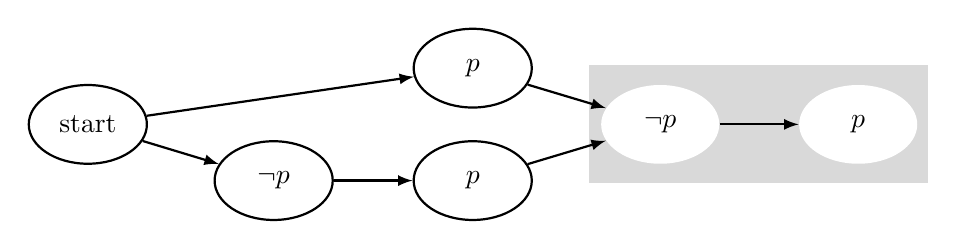
\begin{tikzpicture}
        \node[draw, thick, fill=white, shape=ellipse, style={minimum width=1.5cm, minimum height=1cm}] (p1) {\!\!\!$p$\!\!\!};
        \node[draw, thick, fill=white, shape=ellipse, style={minimum width=1.5cm, minimum height=1cm}] (p2) [below=0.4cm of p1] {\!\!\!$p$\!\!\!};
        \node[draw, thick, fill=white, shape=ellipse, style={minimum width=1.5cm, minimum height=1cm}] (p3) [left= 1cm of p2] {\!\!\!$\lnot p$\!\!\!};
        \node (m) at ($(p1)!0.5!(p2)$) {};
        \node[shape=rectangle, fill=gray!30!white, style={minimum width=4.3cm, minimum height=1.5cm}] (g) [right= 1.35cm of m] {};

        \node[fill=white, shape=ellipse, style={minimum width=1.5cm, minimum height=1cm}] (p4) [right= 1.5cm of m] {\!\!\!$\lnot p$\!\!\!};
        \node[fill=white, shape=ellipse, style={minimum width=1.5cm, minimum height=1cm}] (p5) [right= 1cm of p4] {\!\!\!$p$\!\!\!};
        \node[draw, thick, fill=white, shape=ellipse, style={minimum width=1.5cm, minimum height=1cm}] (s) [left= 4cm of m] {\!\!\!start\!\!\!};
        \draw[thick] (s) edge[-latex] (p1) (s) edge[-latex] (p3) (p3) edge[-latex] (p2) (p1) edge[-latex] (p4) (p2) edge[-latex] (p4) (p4) edge[-latex] (p5);

        \end{tikzpicture}
   %     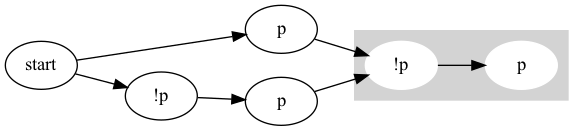
\includegraphics[scale=0.4]{examples/ex2/ex2.png}
        \caption{Example timeline for specification ``$p$ oscillates every time step''}
        \label{fig:ex2}
    \end{figure}
\end{example}

\begin{example}
    In \cref{fig:ex15}, one can reason about one timeline: the atomic proposition $a$ is false for finitely many time steps as signified by two nodes with $!a$ separated by $\cdots$ (could also be zero time step); followed by one node with $a$ which substantiates the specification of ``$a$ eventually true''; once $a$ is true at some point, the later time steps can behave arbitrarily as signified by the infinite run of $1$ (true) in the grey box.
    \begin{figure}[!h]
        \centering
        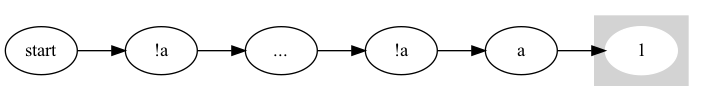
\includegraphics[scale=0.4]{examples/ex15/ex15.png}
        \caption{Example timeline for specification ``$a$ is eventually true''}
        \label{fig:ex15}
    \end{figure}
\end{example}

\section{Algorithm}
On a high level, our algorithm of converting \ltl\ formulas into timeline visualization works as follows:
\begin{enumerate}
    \item Convert the given \ltl\ formula to its corresponding \Buchi automata % (as detailed in \cref{ltl2aut})
    \item Derive the $\omega$-regular expression corresponding to the \Buchi automata % (in \cref{aut2regex})
    \item Simplify the derived $\omega$-regular expression % (in \cref{regex-simplify})
    \item Visualize the $\omega$-regular expression according to its structure %(in \cref{regex2timeline})
\end{enumerate}
\begin{figure}[!h]
    \centering
    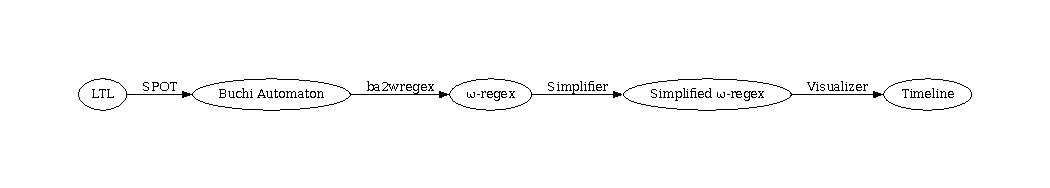
\includegraphics[width=\textwidth]{img/algorithm_outline.pdf}
    \caption{Algorithm outline}
    \label{fig:algo}
\end{figure}

\subsection{LTL to BA} \label{ltl2aut}
The automata-theoretic approach \cite{ORBi-a8d60ab6-1101-4434-9511-c01ea4e5a15b} of studying \ltl\ (i.e. reducing \ltl\ formulas to their corresponding \Buchi automata) has been well-studied. Many algorithms and optimizations have been studied such as \cite{DGV99, F03}. Our tool \tool uses SPOT~\cite{Dur22}\footnote{For our tool, we use SPOT version 2.11.} for this step, which provides an implementation of the translation from \ltl\ formulas to \Buchi automata.

\subsection{BA to $\omega$-regex} \label{aut2regex}
We translate \Buchi automata to $\omega$-regular expressions by first finding the regular expressions for paths from the start state to some final state (say $r_\mathrm{sf}$), and for those for paths for looping from the final state back to itself (say $r_\mathrm{ff}$), and finally combining those to form the $\omega$-expression for valid runs ($\bigplus_{f\in F} r_\mathrm{sf}r_\mathrm{ff}^\omega$). The regular expressions for finite paths are in turn found by iteratively deleting interior nodes in digraph of the automaton.

The algorithm is outlined below (see Algorithms 1 - 4). %\cref{alg:ba2wregex}

\begin{algorithm}[h!]
    \caption{reduce\_dfa}
    \begin{algorithmic}
        \Require ($G, v$), a DFA with state $v$ that is not initial or final
        \Ensure Deletes state $v$ from $G$ while ensuring the same language is recognized
        \For{ every $u\xrightarrow{r_\mathrm{in}} v, v \xrightarrow{r_\mathrm{out}} w$ }
            \If {$v$ has a self-edge  $v\xrightarrow{r_\mathrm{loop}}v$}
                \State replace edges $u\xrightarrow{r_\mathrm{in}} v, v \xrightarrow{r_\mathrm{out}} w$ with $u \xrightarrow{r_\mathrm{in} r_\mathrm{loop}* r_\mathrm{out}} w$
            \Else
                \State replace edges $u\xrightarrow{r_\mathrm{in}} v, v \xrightarrow{r_\mathrm{out}} w$ with $u \xrightarrow{r_\mathrm{in}  r_\mathrm{out}} w$
            \EndIf
        \EndFor
	\State delete node $v$ from $G$
        %\State \Return the reduced graph $G$
    \end{algorithmic}
\end{algorithm}

\begin{algorithm}[h!]
    \caption{dfa2regex}
    \begin{algorithmic}
        \Require ($G, s, f$), a DFA with initial state $s$ and final state $f$
        \Ensure The regular expression corresponding to all paths from $s$ to $f$
        % WHile there exists any edge except r_sf
        \While{ there exists an interior vertex $v$ }
            \State reduce\_dfa($G, v$)
            \State combine multiedges, i.e. $r1 : u \to w, r2 : u \to w$  to $r1 | r2 : u \to w$
        \EndWhile
        \State \Return $(r_\mathrm{ss}| r_\mathrm{sf} r_\mathrm{ff}^* r_\mathrm{fs})^* r_\mathrm{sf} r_\mathrm{ff}$
        % if called by first visit, this is r_\mathrm{ss}* r_\mathrm{sf}
        % if called by ba2wregex, s=f, this is r_\mathrm{ff}
        % consider modularizing fns differently
        % \State \Return regexp labelling the edge $s\to f$
    \end{algorithmic}
\end{algorithm}

\begin{algorithm}[h!]
    \caption{dfa2regex\_firstvisit}
    \begin{algorithmic}
        \Require ($G, s, f$), a DFA with initial state $s$ and final state $f$
        \Ensure The regular expression of all paths from $s$ reaching $f$ for the first time
        \State delete all out edges from $f$ in $G$
        \State \Return dfa2regex($G, s, f$)
    \end{algorithmic}
\end{algorithm}

\begin{algorithm}[h!]
    \label{alg:ba2wregex}
    \caption{ba2wregex}
    \begin{algorithmic}
        \Require $G$, a \Buchi automaton
        \Ensure The $\omega$-regular expression recognized by $G$
        \State \Return $\bigcup_{f \in F}\left(\text{dfa2regex\_firstvisit}(G, s, f)\text{\^{}dfa2regex}(G, f, f) \right) $
    \end{algorithmic}
\end{algorithm}

\subsection{$\omega$-regex simplification} \label{regex-simplify}

The $\omega$-regular expression generated in \cref{aut2regex} may not be the ``simplest'' for the purpose of visualizing the timeline. We have observed multiple patterns in the resulting $\omega$-regular expression that could be simplified. For example, an $\omega$-regular expression in the form of $r^*r^{\omega}$ represents the same timeline as $r^{\omega}$, but the latter is more intuitive. For this purpose, we devised some simplification rules in our tool, based on our observation of common patterns in the generated $\omega$-regular expression.

\paragraph*{Rule-based simplification}
Here we show a demonstrating subset of simplification rules we encoded.
\begin{alignat*}{2}
        & r_1 + r_1r_2^* && \Longrightarrow r_1r_2^* \\
        & r + r && \Longrightarrow r \\
        & r_1 + r_2^*r_1 && \Longrightarrow r_2^*r_1 \\
        & (r^*)^{\omega} && \Longrightarrow r^{\omega} \\
        & (r_1r_2^*)r_2^{\omega} && \Longrightarrow r_1r_2^{\omega} \\
        & (r_1r_2)r_2^{\omega} && \Longrightarrow r_1r_2^{\omega} \\
        & r^*r^{\omega} && \Longrightarrow r^{\omega} \\
        & rr^{\omega} && \Longrightarrow r^{\omega}
\end{alignat*}

\paragraph*{Result of simplification}
Those simplification rules lead to more intuitive representation of timelines. Here we demonstrate their effects using an example.

\begin{example}
    The formula $\Phi = \always (a \limplies \eventually (\neg a))$ generates un-simplified $\omega$-regular expression $((!a) | (aa^*(!a)))((!a) | (aa^*(!a)))^{\omega}$, and simplified version $((!a) | (aa^*(!a)))^{\omega}$, which corresponds to the two timelines in \cref{fig:unsimplified} and \cref{fig:simplified}.
    \begin{figure}[h!]
        \centering
                \resizebox{\textwidth}{!}{
        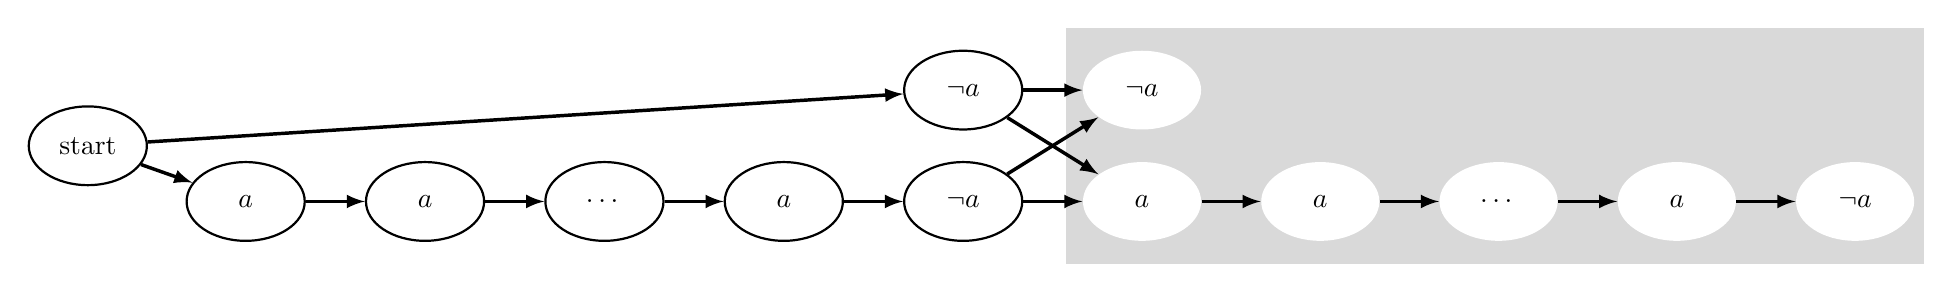
\begin{tikzpicture}
        \node[fill=white, shape=ellipse, style={minimum width=1.5cm, minimum height=1cm}] (a1) {\!\!\!$\lnot a$\!\!\!};
        \node[fill=white, shape=ellipse, style={minimum width=1.5cm, minimum height=1cm}] (a2) [below=0.4cm of a1] {\!\!\!$a$\!\!\!};
        \node (m) at ($(a1)!0.5!(a2)$) {};
        \node[shape=rectangle, fill=gray!30!white, style={minimum width=10.9cm, minimum height=3cm}] (g) [right= -1.1cm of m] {};
        \node[fill=white, shape=ellipse, style={minimum width=1.5cm, minimum height=1cm}] (a1) {\!\!\!$\lnot a$\!\!\!};
        \node[fill=white, shape=ellipse, style={minimum width=1.5cm, minimum height=1cm}] (a2) [below=0.4cm of a1] {\!\!\!$a$\!\!\!};
        \node[fill=white, shape=ellipse, style={minimum width=1.5cm, minimum height=1cm}] (a3) [right= 0.75cm of a2] {\!\!\!$a$\!\!\!};
        \node[fill=white, shape=ellipse, style={minimum width=1.5cm, minimum height=1cm}] (a4) [right= 0.75cm of a3] {\!\!\!$\dots$\!\!\!};
        \node[fill=white, shape=ellipse, style={minimum width=1.5cm, minimum height=1cm}] (a5) [right= 0.75cm of a4] {\!\!\!$a$\!\!\!};
        \node[fill=white, shape=ellipse, style={minimum width=1.5cm, minimum height=1cm}] (a6) [right= 0.75cm of a5] {\!\!\!$\lnot a$\!\!\!};
        \node[draw, thick, fill=white, shape=ellipse, style={minimum width=1.5cm, minimum height=1cm}] (s) [left= 12.5cm of m] {\!\!\!start\!\!\!};

        \node[draw, thick, fill=white, shape=ellipse, style={minimum width=1.5cm, minimum height=1cm}] (a7) [left= .75cm of a1] {\!\!\!$\lnot a$\!\!\!};
        \node[draw, thick, fill=white, shape=ellipse, style={minimum width=1.5cm, minimum height=1cm}] (a8) [left= .75cm of a2] {\!\!\!$\lnot a$\!\!\!};
        \node[draw, thick, fill=white, shape=ellipse, style={minimum width=1.5cm, minimum height=1cm}] (a9) [left= .75cm of a8] {\!\!\!$a$\!\!\!};
        \node[draw, thick, fill=white, shape=ellipse, style={minimum width=1.5cm, minimum height=1cm}] (a10) [left= .75cm of a9] {\!\!\!$\dots$\!\!\!};
        \node[draw, thick, fill=white, shape=ellipse, style={minimum width=1.5cm, minimum height=1cm}] (a11) [left= .75cm of a10] {\!\!\!$a$\!\!\!};
        \node[draw, thick, fill=white, shape=ellipse, style={minimum width=1.5cm, minimum height=1cm}] (a12) [left= .75cm of a11] {\!\!\!$a$\!\!\!};


        \draw[thick, line width=1.25] (s) edge[-latex] (a12) (s) edge[-latex] (a7) (a2) edge[-latex] (a3) (a3) edge[-latex] (a4) (a4) edge[-latex] (a5) (a5) edge[-latex] (a6);
        \draw[thick, line width=1.25] (a12) edge[-latex] (a11) (a11) edge[-latex] (a10) (a10) edge[-latex] (a9) (a9) edge[-latex] (a8) (a8) edge[-latex] (a1) (a8) edge[-latex] (a2) (a7) edge[-latex] (a1) (a7) edge[-latex] (a2);

        \end{tikzpicture}}
%        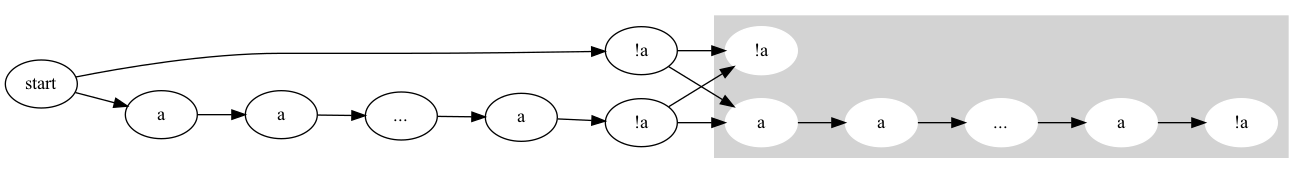
\includegraphics[scale=0.3]{examples/ex9/ex9-unsimplified.png}
        \caption{Timeline for un-simplified $\omega$-regular expression $((!a) | (aa^*(!a)))((!a) | (aa^*(!a)))^{\omega}$}
        \label{fig:unsimplified}
    \end{figure}
    \begin{figure}[h!]
        \centering
        \resizebox{.8\textwidth}{!}{
        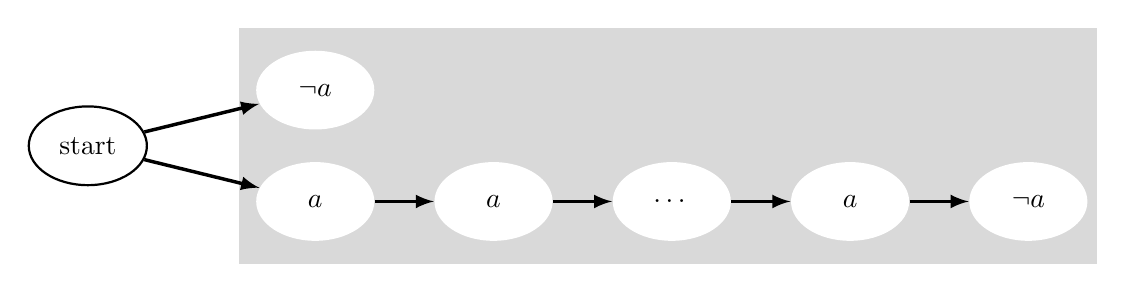
\begin{tikzpicture}
        \node[fill=white, shape=ellipse, style={minimum width=1.5cm, minimum height=1cm}] (a1) {\!\!\!$\lnot a$\!\!\!};
        \node[fill=white, shape=ellipse, style={minimum width=1.5cm, minimum height=1cm}] (a2) [below=0.4cm of a1] {\!\!\!$a$\!\!\!};
  %      \node[draw, thick, fill=white, shape=ellipse, style={minimum width=1.5cm, minimum height=1cm}] (p3) [left= 1cm of p2] {\!\!\!$\lnot p$\!\!\!};
        \node (m) at ($(a1)!0.5!(a2)$) {};
        \node[shape=rectangle, fill=gray!30!white, style={minimum width=10.9cm, minimum height=3cm}] (g) [right= -1.1cm of m] {};
        \node[fill=white, shape=ellipse, style={minimum width=1.5cm, minimum height=1cm}] (a1) {\!\!\!$\lnot a$\!\!\!};
        \node[fill=white, shape=ellipse, style={minimum width=1.5cm, minimum height=1cm}] (a2) [below=0.4cm of a1] {\!\!\!$a$\!\!\!};
        \node[fill=white, shape=ellipse, style={minimum width=1.5cm, minimum height=1cm}] (a3) [right= 0.75cm of a2] {\!\!\!$a$\!\!\!};
        \node[fill=white, shape=ellipse, style={minimum width=1.5cm, minimum height=1cm}] (a4) [right= 0.75cm of a3] {\!\!\!$\dots$\!\!\!};
        \node[fill=white, shape=ellipse, style={minimum width=1.5cm, minimum height=1cm}] (a5) [right= 0.75cm of a4] {\!\!\!$a$\!\!\!};
        \node[fill=white, shape=ellipse, style={minimum width=1.5cm, minimum height=1cm}] (a6) [right= 0.75cm of a5] {\!\!\!$\lnot a$\!\!\!};
        \node[draw, thick, fill=white, shape=ellipse, style={minimum width=1.5cm, minimum height=1cm}] (s) [left= 2cm of m] {\!\!\!start\!\!\!};
        \draw[thick, line width=1.25] (s) edge[-latex] (a1) (s) edge[-latex] (a2) (a2) edge[-latex] (a3) (a3) edge[-latex] (a4) (a4) edge[-latex] (a5) (a5) edge[-latex] (a6);
        \end{tikzpicture}}
  %      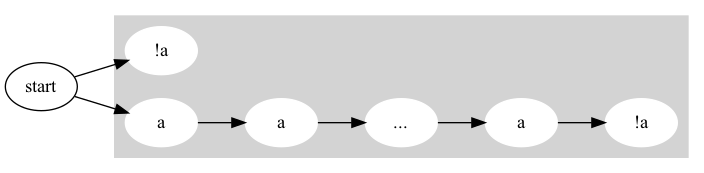
\includegraphics[scale=0.3]{examples/ex9/ex9.png}
        \caption{Timeline for simplified $\omega$-regular expression $((!a) | (aa^*(!a)))^{\omega}$}
        \label{fig:simplified}
    \end{figure}
\end{example}

\begin{remark}
    Both simplified and un-simplified $\omega$-regular expression would generate correct timeline representations. Correct as they faithfully represent the set of satisfying traces of the original \ltl\ formula $\Phi$. Nonetheless, we, as human users, oftentimes find the simplified version more intuitive to reason about.
\end{remark}

\subsection{$\omega$-regex to timeline} \label{regex2timeline}
Our tool uses Graphviz~\cite{Ellson2001GraphvizO} to achieve the timeline visualization step. By construction of our algorithm, every $\omega$-regular expression is in the form of
\[
    A_1A_2^{\omega} + A_3A_4^{\omega} + \cdots + A_{2n-1}A_{2n}^{\omega}
\]
where $A_i$ are regular expressions, and $A_{2i-1}$ could be $\epsilon$. On a high level, for each of regular expression $A_i$, we visualize it as a set of accepted input. We view each union operator as parallel timelines, and each $A_{2i-1}$ is concatenated with $A_{2i}$ repeated infinitely many times, as represented in the grey box. \cref{fig:timeline} presents a generic timeline resulting from this form of construction.
\begin{figure}[h!]
    \centering
    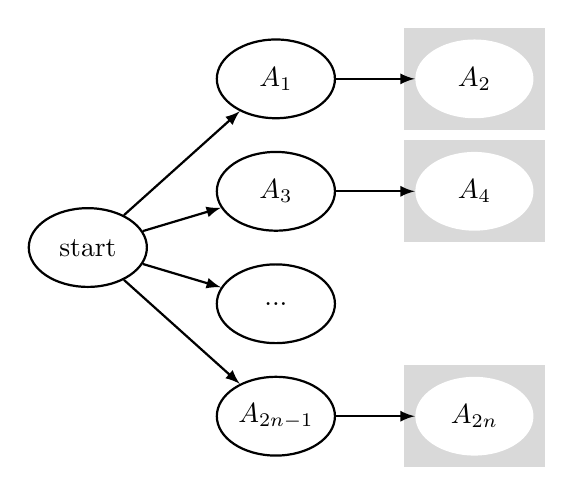
\begin{tikzpicture}
    \node[draw, thick, fill=white, shape=ellipse, style={minimum width=1.5cm, minimum height=1cm}] (a1) {$A_1$};
    \node[shape=rectangle, fill=gray!30!white, style={minimum width=1.8cm, minimum height=1.3cm}] (a2g) [right= 0.85cm of a1] {};
    \node[fill=white, shape=ellipse, style={minimum width=1.5cm, minimum height=1cm}] (a2) [right= 1cm of a1] {$A_2$};
    \node[draw, thick, shape=ellipse, style={minimum width=1.5cm, minimum height=1cm}] (a3) [below= 0.4cm of a1] {$A_3$};
    \node[shape=rectangle, fill=gray!30!white, style={minimum width=1.8cm, minimum height=1.3cm}] (a4g) [right= 0.85cm of a3] {};
    \node[fill=white, shape=ellipse, style={minimum width=1.5cm, minimum height=1cm}] (a4) [right= 1cm of a3] {$A_4$};
    \node[draw, thick, fill=white, shape=ellipse, style={minimum width=1.5cm, minimum height=1cm}] (a5) [below= 0.4cm of a3] {...};
    \node[draw, thick, fill=white, shape=ellipse, style={minimum width=1.5cm, minimum height=1cm}] (a7) [below= 0.4cm of a5] {\!\!\!$A_{2n-1}$\!\!\!};
    \node[shape=rectangle, fill=gray!30!white, style={minimum width=1.8cm, minimum height=1.3cm}] (a8g) [right= 0.85cm of a7] {};
    \node[fill=white, shape=ellipse, style={minimum width=1.5cm, minimum height=1cm}] (a8) [right= 1cm of a7] {\!\!\!$A_{2n}$\!\!\!};
    \node (m) at ($(a1)!0.5!(a7)$) {};
    \node[draw, thick, fill=white, shape=ellipse, style={minimum width=1.5cm, minimum height=1cm}] (s) [left= 1.5cm of m] {\!\!\!\!start\!\!\!\!};
    \draw[thick] (s) edge[-latex] (a1) (s) edge[-latex] (a3) (s) edge[-latex] (a5) (s) edge[-latex] (a7);
    \draw[thick] (a1) edge[-latex] (a2) (a3) edge[-latex] (a4) (a7) edge[-latex] (a8);
    \end{tikzpicture}
%    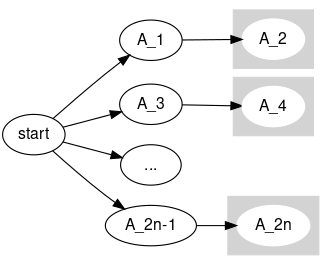
\includegraphics[scale=0.5]{img/timeline.png}
    \caption{Generic timeline construction from $A_1A_2^{\omega} + A_3A_4^{\omega} + \cdots + A_{2n-1}A_{2n}^{\omega}$}
    \label{fig:timeline}
\end{figure}

\section{Theoretical Analyses} \label{sec:analysis}
\subsection{Correctness of Regex Translation}
\begin{lemma}
    % reduce_dfa does its input to output behaviour
    For any DFA $G$ and any state $v$ in $G$ that is neither a start state or a final state, \textbf{reduce\_dfa}$(G, v)$ preserves the regular language accepted by $G$
\end{lemma}
\begin{proof}
    Let $G'$ be the graph of $G$ post reduction by the application of \textbf{reduce\_dfa}$(G, v)$. We show that the trace of every path accepted by $G$ is also accepted by $G'$. Suppose a path accepted by $G$ does not pass through $v$, clearly this is true. Else, suppose it passes through $v$, since $v$ is an interior node, $v$ cannot be the first or last in the path. Thus, for every pass through $v$, let $u\neq v$ be the last node passed before entering $v$, and likewise $w$ be the first node after exiting $v$. We show that the regular language of sub-traces from $u$ to $w$ in $G$ (shown in \cref{fig:uvw-dfa}) is identical to that in $G'$.
    \begin{figure}[h!]
        \centering
        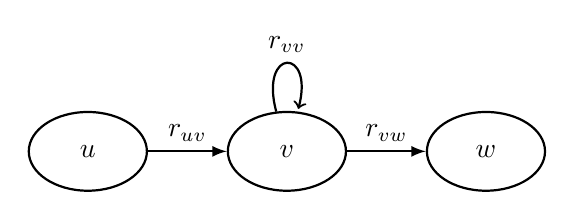
\begin{tikzpicture}
	\node[draw, thick, shape=ellipse, style={minimum width=1.5cm, minimum height=1cm}] (u) {$u$};
	\node[draw, thick, shape=ellipse, style={minimum width=1.5cm, minimum height=1cm}] (v) [right=of u] {$v$};
	\node[draw, thick, shape=ellipse, style={minimum width=1.5cm, minimum height=1cm}] (w) [right=of v] {$w$};
	\draw[thick] (u) edge["$r_{uv}$",-latex] (v) (v) edge["$r_{vv}$",-latex,loop above] (v) (v) edge["$r_{vw}$",-latex] (w);
        \end{tikzpicture}
 %       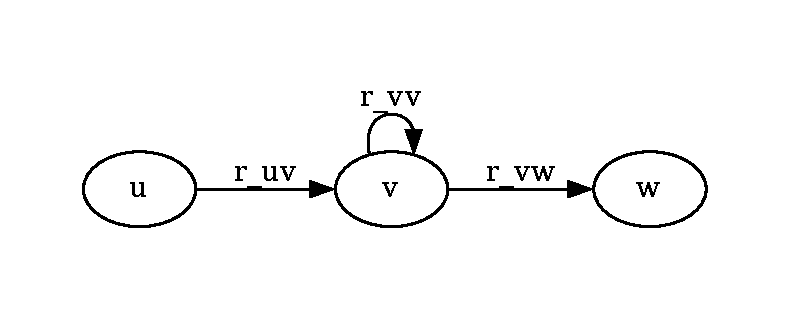
\includegraphics[scale=0.75]{img/uvw_dfa.pdf}
        \caption{A path from $u$ to $w$ in $G$}
        \label{fig:uvw-dfa}
    \end{figure}
    Suppose there is no loop at $v$, the path from $u$ to $w$ must simply be $u\xrightarrow{r_{uv}}v\xrightarrow{r_{vw}}w$, with the trace $r=r_{uv}r_{vw}$. If there is a loop edge $r_{vv}$, this edge can be traveled any number of times before exiting $v$, thus the regular expression is $r=r_{uv}r_{vv}^*r_{vw}$. This edge $u\xrightarrow{r}w$ is added in $G'$. Thus, for every path accepted by $G$, for every subpath entering and exiting $v$ from some $u$ to $w$, there exists a corresponding subpath from $u$ to $w$ in $G'$, and thus a corresponding path accepted by $G'$.
\end{proof}

\begin{lemma}
    For any DFA $G$ with start state $s$ and (exactly one) final state $f$, \textbf{dfa2regex}$(G, s, f)$ outputs the regular expression of all paths from $s$ to $f$ (i.e., the language accepted by $G$)
\end{lemma}
\begin{proof}
    The while loop clearly terminates since the number of interior nodes is strictly decreasing, and upon termination, $G$ is a DFA containing only the nodes $s$ and $f$. Now, every non-terminal visit from $s$ to $f$ and back to $s$, can be replaced by an edge $s\xrightarrow{r_\mathrm{sf}r_\mathrm{ff}^* r_\mathrm{fs}} s$, instead of the edge $f\to s$. This DFA yields the regular language $(r_\mathrm{ss}|r_\mathrm{sf}r_\mathrm{ff}^* r_\mathrm{fs})^* r_\mathrm{sf} r_\mathrm{ff}$, as outputted by the algorithm.
\end{proof}

\begin{lemma}
    For any DFA $G$ with start state $s$ and (exactly one) final state $f$, \textbf{dfa2regex\_firstvisit}$(G, s, f)$ outputs the regular expression of all paths from $s$ to $f$, visiting $f$ for the first time.
\end{lemma}
\begin{proof}
    Let $G'$ be $G$ with all out-edge (including loops) from $f$ deleted. We claim that $L(G')$ is equal to the language $L'$ of all paths from $s$ reaching $f$ for the first time.

    First we show $L(G') \subseteq L'$, i.e., every path accepted by $G'$ starts in $s$ and ends by reaching $f$ for the first time. Since $s$ and $f$ are the initial and final states of $G'$ respectively, clearly every path accepted by $G$ must start in $s$ and end in $f$. Further, as $f$ has no out-edges in $G$, any accepted path must end immediately once it reaches $f$. Thus it must end once it reaches $f$ for the first time.

    Also, we show $L' \subseteq L(G')$, i.e., every path starting in $s$ and ending by $f$ reaching $f$ for the first time is accepted by $G'$. If a path contains an out-edge of $f$, it cannot be in $L'$ as the trace continues beyond the first time step at $f$. Thus, every trace in $L'$ only uses edges in $G'$, and is thus accepted by $G$ iff it is accepted by $G'$.
\end{proof}

\begin{theorem}
    For any \Buchi automaton $G$ with start state $s$ and final states $F$, \textbf{ba2wregex}$(G)$ outputs the $\omega$-regular language accepted by $G$
\end{theorem}
\begin{proof}
    We show that
    \[
        L = \bigcup_{f\in F} \textbf{dfa2regex}(G, s, f) \verb|^| \left(\textbf{dfa2regex\_firstvisit}(G, f, f)\right)^\omega
    \]
    and the $\omega$-language accepted by $G$, $L_\omega(G)$ are identical.

    First, $L\subseteq L_\omega(G)$ since for every infinite run in $L$, clearly by definition of $L$, there is some $f\in F$ such that passes through $f$ infinitely often. The converse is true as well: for every infinite run $q_0, q_1, \dots$ accepted by $G$, then $q_0 = s$ and by definition of the accepting language, there is some accepting state $f$, passed through infinitely often, thus the run is in $\textbf{dfa2regex}(G, s, f)$ \verb|^| $\left(\textbf{dfa2regex\_firstvisit}(G, f, f)\right)^\omega$
\end{proof}
\subsection{Correctness of Rewrite Rules}
\begin{lemma}
    For all regular expressions $r_1, r_2, r$, each of the following rewrite rules preserve the regular or $\omega$-regular language represented by the expressions:
    \begin{alignat}{2}
        & r_1 + r_1r_2^* && \Longrightarrow r_1r_2^* \\
        & r + r && \Longrightarrow r \\
        & r_1 + r_2^*r_1 && \Longrightarrow r_2^*r_1 \\
        & (r^*)^{\omega} && \Longrightarrow r^{\omega} \\
        & (r_1r_2^*)r_2^{\omega} && \Longrightarrow r_1r_2^{\omega} \\
        & (r_1r_2)r_2^{\omega} && \Longrightarrow r_1r_2^{\omega} \\
        & r^*r^{\omega} && \Longrightarrow r^{\omega} \\
        & rr^{\omega} && \Longrightarrow r^{\omega}
    \end{alignat}
\end{lemma}

The soundness of each of these translations can be proven by reasoning about the  semantics detailed in \cref{def:omega-semantics}. A full proof is not provided here.

\section{Tool showcase} \label{sec:tool-showcase}
To demonstrate the result of our tool, we present two examples, one from a real-world model checking example from Zhao and Rozier~\cite{ZR14} and one from a randomly generated \ltl\ formula.

\begin{example} \label{example:air}
    Zhao and Rozier~\cite{ZR14} presents a model verification specification says ``[i]f a TSAFE command is sent to an aircraft, controller/AutoResolver should then hand off the control of this aircraft'' which corresponds to \ltl\ formula
    \begin{align*}
        \always (\texttt{tsafe.TSAFE\_command1} \land \texttt{controller.CTR\_control\_1} \\
        \limplies \nextt (\neg \texttt{controller.CTR\_control\_1}))
    \end{align*}
    For simplicity, we swap the concrete atomic proposition to $a,b$ and get
    \[
        \always (a \land b \limplies \nextt (\neg b))
    \]
    For this \ltl\ formula, our tool generates the timeline representation in \cref{fig:ex14}.
    \begin{figure}[h!]
        \centering
        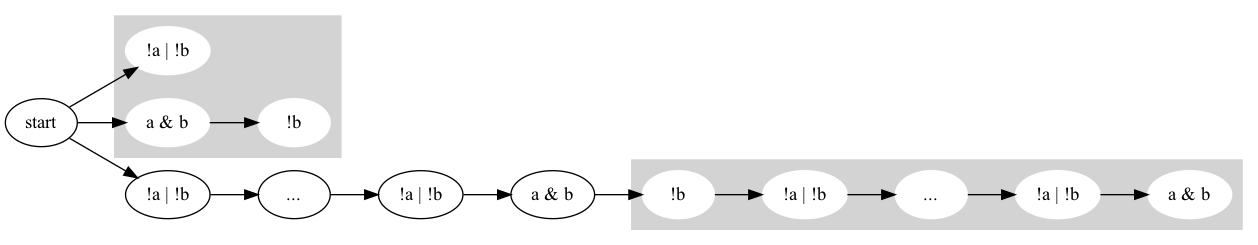
\includegraphics[scale=0.3]{examples/ex14/ex14.png}
        \caption{Timeline for $\always (a \land b \limplies \nextt (\neg b))$}
        \label{fig:ex14}
    \end{figure}
\end{example}

\begin{example}
    Spot~\cite{SPOT-online} presents command-line tool for random \ltl\ formula generator \texttt{randltl}~\cite{duret.13.atva}. The following \ltl\ formula is generated from this tool.
    \[
    p_2 \land (\eventually \always p_0 \weakrelease \nextt(\always p_1 \land ((p_0 \limplies p_2 \land p_2 \limplies p_0) \stronguntil \eventually p_0)))
    \]
    This formula is reasonably complicated, and hard for human to reason about directly. For this \ltl\ formula, our tool generates the timeline representation in \cref{fig:ex13}.
    \begin{figure}[h!]
        \centering
        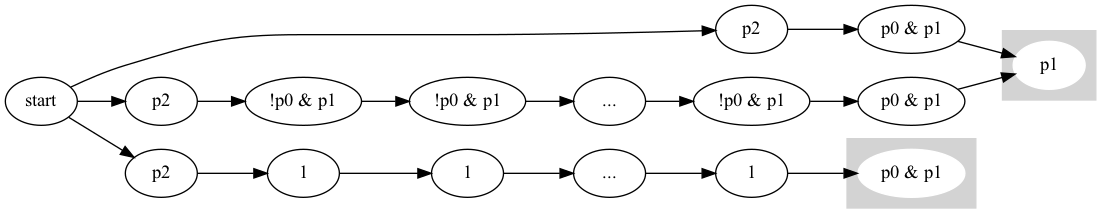
\includegraphics[scale=0.3]{examples/ex13/ex13.png}
        \caption{Timeline for $p_2 \land (\eventually \always p_0 \weakrelease \nextt(\always p_1 \land ((p_0 \limplies p_2 \land p_2 \limplies p_0) \stronguntil \eventually p_0)))$}
        \label{fig:ex13}
    \end{figure}
\end{example}
\begin{remark}
    These two examples show that our tool can generate reasonably clear diagrams for both real-world formula and randomly generated formula.
\end{remark}

\section{Playing it out} \label{sec:playing}%KYR: may swap order with the next section on artifact availability?

We quantify the usability and performance of \tool by compiling an extensive set of \ltl\ formulas used in the analysis of real-life systems, defining timeline metrics, and characterizing the result of visualizing the set of real-life \ltl\ formulas over those metrics.
% We release the set of real-life \ltl\ formulas as a benchmark set for the research community. 
Our experimental evaluation conclusively demonstrates that \tool scales to provide helpful visualizations of \ltl\ formulas written by humans.


\subsection{Timeline Metrics}
\label{sec:metrics}

%KYR: Define size, length, height, complexity, etc. here.

We use two measures of complexity for timeline visualizations: timeline length and star height.

We use timeline length, defined below, to capture the length of our timeline visualization graphs. Since Kleene stars are the trickiest operator to depict in timelines, we also use star height, a well-studied measure for the structural complexity of regular expressions, to measure the complexity of our visualizations.

\begin{definition}[Timeline Length]
    We define the timeline length of a regular expression $\tllen(A)$ recursively as follows
    \begin{align*}
        \tllen(\emptyset)   &= -\infty\\
        \tllen(\epsilon)        &= 0\\
        \tllen(a)           &= 1\\
        \tllen(A_1 A_2)     &= \tllen(A_1) + \tllen(A_2)\\
        \tllen(A_1 + A_2)   &= \max(\tllen(A_1, A_2))\\
        \tllen(A^*)         &= 2\tllen(A) + 1
    \end{align*}
    We also extend this definition to $\omega$-regular expressions as follows
    \begin{align*}
        \tllen(A^\omega)    &= \tllen(A)\\
        \tllen(AB)          &= \tllen(A) + \tllen(B)\\
        \tllen(B_1 + B_2)   &= \max(\tllen(B_1), \tllen(B_2))
    \end{align*}
    This quantity $\tllen$ captures the length of the longest path in our timeline graph visualization.
\end{definition}

\begin{definition}[Star height]
    We define the star height of regular and $\omega$-regular expressions to be the star-nesting depth in the (unsimplified) expression. Namely,
    \begin{align*}
        h(\emptyset) = h(\epsilon) = h(a) &= 0\\
        h(A_1 A_2) = h(A_1 + A_2) &= \max(h(A_1), h(A_2))\\
        h(A^*) &= 1 + h(A)\\
        h(A^\omega) &= h(A)\\
        h(A B) &= \max(h(A), h(B))\\
        h(B_1 + B_2) &= \max(h(B_1), h(B_2))
    \end{align*}

\end{definition}

\subsection{Experimental Analysis} %We could come up with a less-generic name for this, which would be nicer...

%KYR: Here we nicely show (with pictures as much as possible) all of the individual statistics and results we gathered (note aggregation occurs below).
\paragraph{Real-world datasets} We study the feasibility of our tool on a benchmark suite of LTL formulas gathered from real world use cases. 

We gather a test suite of 91 formulas used in real-world requirement specification. We take $6$ specifications from NASA's Automated Airspace Concept (AAC)\cite{GCMTR16}. We also collect formulas from the Acacia suite of examples \cite{RV10}. We reap $85$ formulas from the suit of $23$ examples, by generating seperate visualizations for each line of specification. % We choose to visualize each formula specifically, rather than complete specifications, as 

We run \texttt{ltl2regex} on these $91$ examples, the tool completes execution (within timeout of $20$s) on $87$. Within the $87$, two examples have regular expressions of star height $8$ and are intractible to generate graph visualizations of. We are able to generate tractible visualization on the $85$, or over $93\%$ of benchmarks tested. The plots of visualization complexity on these formula are provided below in \cref{fig:real-world}.


\begin{figure}[h!]
    \centering
    \subfloat{{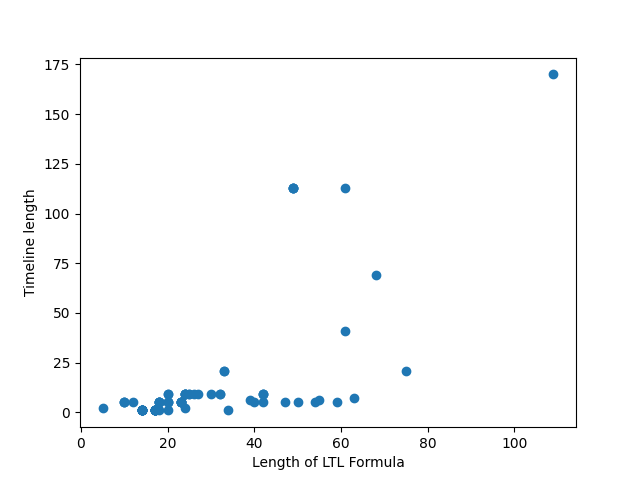
\includegraphics[width=6.5cm]{img/naive-ltl2tl-scatterplot-omit-big-values.png} }}%
    \quad % [\centering label 1]
    \subfloat{{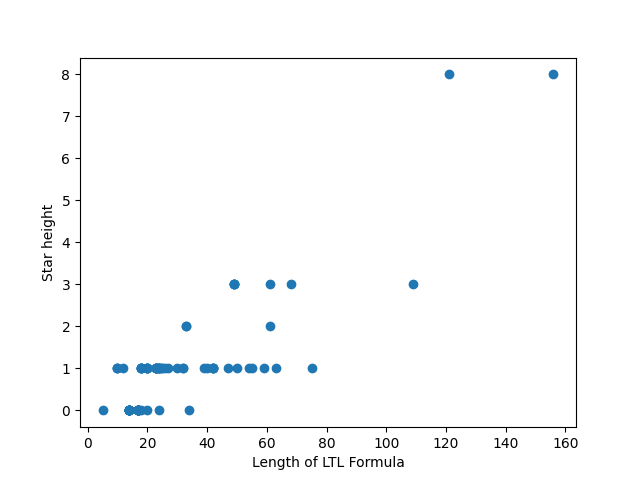
\includegraphics[width=6.5cm]{img/star-height-scatter-plot.png}}}
    \caption{Visualization complexity metrics for formulas collected from Acacia \cite{RV10} and NASA's  AAC \cite{GCMTR16}}
    \label{fig:real-world}
\end{figure}

\paragraph{Scalability}
We measure the scalability of our tool by running it against a set of scalable \ltl\ formulas. We define a scalable \ltl\ formula as one that describes an $n$-bit number using a binary counter \cite{RV10}. As $n$ gets larger, the \ltl\ formula used to encode the $n$-bit counter scales in size, but it remains practical. The result is shown in \cref{fig:scalability}. In this analysis, the timeline length grows approximately exponentially with the number of bits in the counter, which matches the result in Rozier and Vardi \cite{RV10}.

In \cref{fig:scalability}, the x-axis ranges from $1$ to $6$, after which point it hits the $30$ seconds timeout we set, as the timeline length grows exponentially fast.

\begin{figure}[h!]
    \centering
    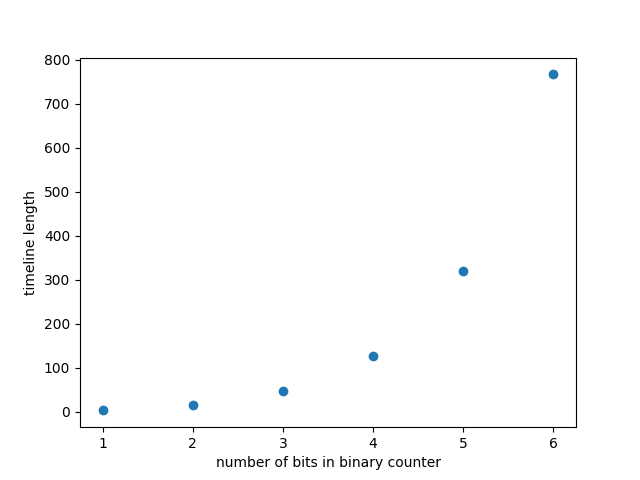
\includegraphics[scale=0.7]{img/scale.png}
    \caption{Scalability measured with binary counter examples from Rozier and Vardi \cite{RV10}}
    \label{fig:scalability}
\end{figure}

% KYR: Here we characterize the size of the timeline as a function of the number of bits of a binary counter for each of the four binary counter \ltl\ formulas. The point is that these four are the only (unboundedly) scalable formulas that describe something real (i.e., they describe a binary counter for any number of bits) that have ever been published in the literature. These would throw off our metrics about the set of real \ltl\ formulas if we included them in there. Thus, we analyze them separately, and can define the timeline size as a function of the number of bits for each of the four formulas. We can give an example or two here, such as two pictures of timelines for a 2-bit and a 3-bit counter from two different formulas, one with U's and one with X's; one with carry and one without (such as a 2-bit w/carry X formula and a 3-bit no carry U formula). The scalable counter formulas are from \cite{RV10}.


%\paragraph{Denouement}
%KYR: aggregate and summarize all experiments here.

%<image>
%caption: For all of the <large number> of real LTL formulas historically used to analyze real systems, \tool efficiently yields usable, readable timeline visualizations.



\section{Artifact availability}
The tool we present in this paper is available at
\[
    \texttt{\url{https://github.com/EULIR/ltl-explainability}}
\]
which comes with two command-line tools, \texttt{ltl2regex} and \tool. The specific usage of the tool can be found  \href{https://github.com/EULIR/ltl-explainability#usage}{here}.

The set of \ltl\ formulas we used to evaluate our tool in \cref{sec:playing} can be found \href{https://github.com/EULIR/ltl-explainability/tree/main/ltl-formulas}{here}.

\section{Discussion}
Based on our results, we propose the following questions for discussions and future works:
\begin{itemize}
    \item Can there be more simplifications methods as described in Section \ref{regex-simplify}? The answer is definitely positive. On one hand, more rule-based simplifications can be discovered by finding more patterns in the generated $\omega$-regular expressions. On the other hand, other simplification are possible: for example, if the generated $\omega$-regular expression is $r_1 + r_2$ where $r_1, r_2$ are not syntactically equivalent (or equivalent up to algebraic rules) $\omega$-regular expressions, but they accepts the same set of infinite-length strings, then we can simplify this down to just $r_1$. This reduce the problem to equivalence test on $\omega$-regular expressions, which is decidable. In the similar vein, many more simplifications can be used, but the question is how efficient are they? In the end, one have to balance trade-off between the efficiency of the tool and the simplicity of the result.
    %\item Our tool is effective at translating a wide range of LTL formulas. Even with LTL formulae with complex nesting structure are represented by relatively readable timeline visualizations.
    \item Can we define timeline more formally so that one can do this process reversely (i.e. a tool that converts timeline representation to its corresponding \ltl\ formula)? That would be a very useful tool in practice. However, a direct reverse of the algorithm we presented in this paper may not be viable.
\end{itemize}

\section{Conclusion}
The Achilles heel of formal verification is specification; formal methods are only as effective at verification as their specifications are at describing the essential properties to verify. Yet, specification remains the biggest bottleneck to the use of formal methods \cite{Roz16}. LTL is one of the most popular specification logics for industrial-scale critical systems; in the space domain alone, it is currently encapsulating specifications for the development of the NASA Lunar Gateway \cite{DBR21}, the Air Force Research Laboratory/Collins Aerospace Spacecraft Collision Avoidance system \cite{HDWF21}, Space Systems Finland's Attitude and Orbit Control Systems (AOCS) \cite{ILLTV13}, and NASA/JPL's Europa Lander Mission Concept \cite{CDRWRWL22} just to name a few. 
 %
Yet the humans that need to use formal verification tools and deeply understand their results struggle to validate that LTL formulas capture the specifications they are meant to capture. A major contributor to LTL's popularity is the propensity of humans to think of requirements in terms of timelines. This inspired the creation of LTL in the first place, as a logic that ``intuitively'' represents timelines. Our work serves to reinforce that connection, enabling visualization of most realistic LTL formulas as timelines. By releasing \tool, we contribute to better validation capabilities for LTL specifications and aid the effort to make formal verification more accessible and wide-spread. 
%We hope that this will assist system designers in formulating error-free specifications and thus improve the effectiveness of verification tools for \ltl.

Future extensions of this work include optimizations to the algorithm and implementation to improve performance and scalability. While we have chosen visual elements that succinctly represent timelines, it would be informative to conduct a study on different possible visualizations and which of the many ways of representing different timeline elements humans find most intuitive. It is possible that factors of context, such as the type of requirement an LTL formula describes, change its optimal timeline representation. 

\appendix
\section{Concrete Syntax of \tool} \label{sec:concrete-syntax}
Recall from \ref{ltl-defn} that we define \ltl\ formula as
\begin{align*}
    \Phi ::= p \mid \neg \Phi \mid \Phi \land \Phi \mid \Phi \lor \Phi \mid \Phi \limplies \Phi \mid \always \Phi \mid \eventually \Phi \mid \nextt \Phi \mid \Phi \stronguntil \Phi \mid \Phi \weakrelease \Phi
\end{align*}
where $p \in \AP$. In our tool \tool, we use the following concrete syntax to represent \ltl\ formulae.
\[
    \begin{array}{c r l l l@{\qquad} l}
         &      & \textit{abstract syntax}              & \textit{concrete syntax}                       & \textit{description} \\
    \Phi & ::=  & p                                     & \texttt{p}                                     & \text{atomic proposition} \\
         & \mid & \neg \Phi                             & \texttt{!} \Phi                                & \text{negation} \\
         & \mid & \Phi \land \Phi                       & \Phi \texttt{ \& } \Phi                        & \text{conjunction} \\
         & \mid & \Phi \lor \Phi                        & \Phi \texttt{ | } \Phi                         & \text{disjunction} \\
         & \mid & \Phi \limplies \Phi                   & \Phi \texttt{ -> } \Phi                        & \text{implication} \\
         & \mid & \always \Phi                          & \texttt{G} \Phi                                & \text{globally} \\
         & \mid & \eventually \Phi                      & \texttt{F} \Phi                                & \text{finally} \\
         & \mid & \nextt \Phi                           & \texttt{X} \Phi                                & \text{next} \\
         & \mid & \Phi \stronguntil \Phi                & \Phi \texttt{ U } \Phi                         & \text{until} \\
         & \mid & \Phi \weakrelease \Phi                & \Phi \texttt{ R } \Phi                         & \text{release} \\
    \end{array}
\]

\bibliographystyle{elsarticle-num}
\bibliography{RelatedWork}


\end{document}


\subsection{Set of Real LTL Formulas}

We collect the \ltl\ formulas from a covering set of publicly-available case studies that use \ltl\ in the analysis of real-life safety-critical systems. As some formulas are redundant (i.e., common properties occur in many different case studies), it is not necessary to include every paper that has ever used \ltl\ in a real setting; we instead opt for the largest and most unique formulas to cover the space of realistic use of \ltl.

Given the tremendous popularity of \ltl\ as a specification language for industrial analysis, surprisingly few real-life system analysis case studies publicly release their \ltl\ formula specifications, largely to protect proprietary system information. We purposely avoid using the random or machine-generated formulas from published benchmarks because the purpose of \tool is helping humans understand and validate \ltl\ formulas. Thus, we gather an extensive, representative set of formulas humans have written or needed to understand. Our \ltl\ formula collection is as follows.

\noindent
\begin{table}[h]
\begin{tabular}{p{3.6in}|c|c}
  \hline
  Purpose & \# formulas & Source \\
  \hline
  Design space for NASA's AAC (Automated Airspace Concept) & 20,250 & \cite{GCMTR16} \\
  \hline
  Safety specifications for Boeing's AIR6110 wheel brake system & & \cite{BCFJKPRT15} \\
  \hline
  Requirements for model checking NASA's AAC high-level architecture & 6 & \cite{ZR14} \\
  \hline
  Real formulas collected from all publicly-available, pre-2011 case studies & 63 & \cite{RV11} \\
  \hline
\end{tabular}
\end{table}


